The desired coordinates are
\begin{align}
\vec{D} &= \frac{1\vec{B}+3\vec{A}}{4} &= \myvec{-1\\7/2}\\
\vec{E} &= \frac{2\vec{B}+2\vec{A}}{4} &= \myvec{0\\5}\\
\vec{F} &= \frac{3\vec{B}+1\vec{A}}{4} &= \myvec{1\\13/2}
\end{align}

The following code plots Fig. \ref{fig:3.6.7}
\begin{lstlisting}
solutions/7/codes/line/point_line/line_division.py
\end{lstlisting}

\begin{figure}[!ht]
\centering
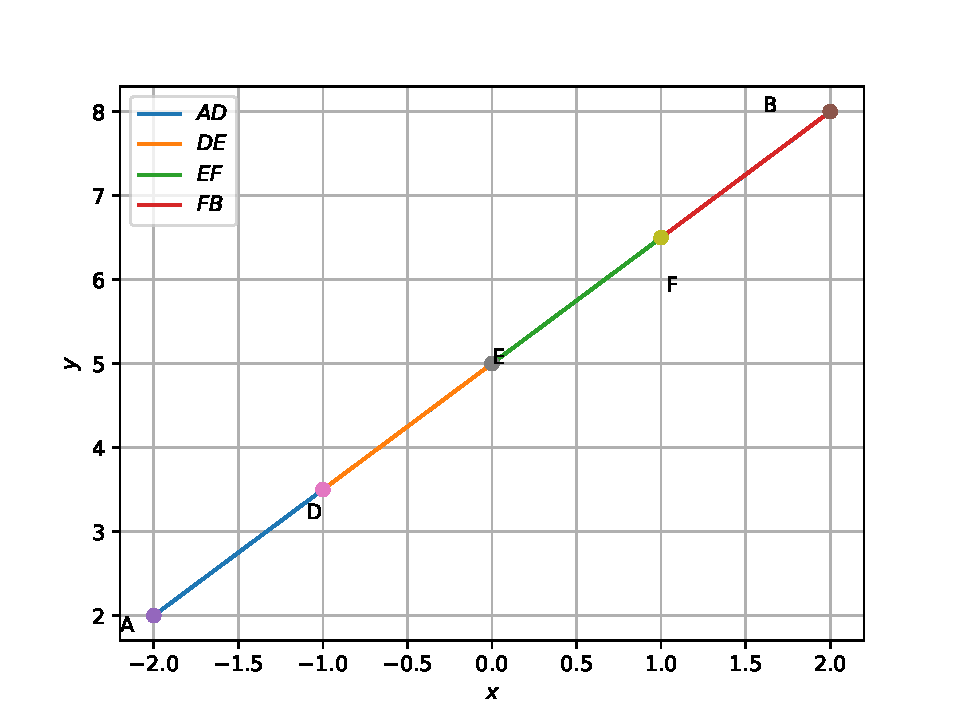
\includegraphics[width=\columnwidth]{./solutions/7/figs/line/point_line/line.eps}
\caption{}
\label{fig:3.6.7}
\end{figure}

